\documentclass[11pt]{article}
\usepackage{fullpage}
\usepackage{amsthm}

\usepackage{amsthm,amsmath,amsfonts,amssymb,amstext,enumitem}
\usepackage{latexsym,ifthen,url,rotating,graphicx}
\usepackage{listings}

\usepackage[usenames,dvipsnames]{color}

% --- -----------------------------------------------------------------
% --- Document-specific definitions.
% --- -----------------------------------------------------------------
\lstset{
    columns=fixed,
    literate={—}{{---}}1 {…}{{...}}1
}

\newcommand{\todo}[1]{{\color{red}[TODO:{#1}]}}

\newtheorem{problem}{Problem}
\newtheorem{fact}{Fact}
\newtheorem{exercise}{Exercise}
\newtheorem{theorem}{Theorem}
\newtheorem{definition}{Definition}
\newtheorem{notation}{Notation}
\newtheorem{lemma}{Lemma}
\newtheorem{example}{Example}

\newcommand{\getsr}
  {{\:\stackrel{\raisebox{-2pt}{${\scriptscriptstyle \hspace{0.2em}\$}$}}
   {\leftarrow}\:}}
\newcommand{\points}[1]{\textbf{({#1} pts)}}

\newcommand{\Colon}{\ : \ }
\newcommand{\st}{\mathsf{state}}
\newcommand{\msgs}{\mathcal{M}}
\newcommand{\ctxts}{\mathcal{C}}
\newcommand{\keys}{\mathcal{K}}
\newcommand{\kg}{\mathcal{K}}
\newcommand{\enc}{E}
\newcommand{\dec}{E^{-1}}
\newcommand{\MAC}{\mathrm{MAC}}
\newcommand{\RMAC}{\mathrm{RMAC}}

\newcommand{\pk}{pk}
\newcommand{\sk}{sk}

\newcommand{\AES}{\mathsf{AES}}

\newcommand{\algorithm}[1]{\textbf{Alg} {#1}}

\newcommand{\calO}{\mathcal{O}}

\newcommand{\dlog}{\mathrm{dlog}}

\newcommand{\Adv}{\mathbf{Adv}}
\newcommand{\AdvPRF}[2]{\Adv^{\mathrm{prf}}_{#1}({#2})}
\newcommand{\AdvCPA}[2]{\Adv^{\mathrm{ind{-}cpa}}_{#1}({#2})}
\newcommand{\AdvCCA}[2]{\Adv^{\mathrm{ind{-}cca}}_{#1}({#2})}
\newcommand{\AdvKR}[2]{\Adv^{\mathrm{kr}}_{#1}({#2})}
\newcommand{\AdvCKR}[2]{\Adv^{\mathrm{ckr}}_{#1}({#2})}
\newcommand{\AdvRMR}[2]{\Adv^{\mathrm{rmr}}_{#1}({#2})}
\newcommand{\AdvCR}[2]{\Adv^{\mathrm{cr}}_{#1}({#2})}
\newcommand{\AdvUFCMA}[2]{\Adv^{\textrm{uf{-}cma}}_{#1}({#2})}
\newcommand{\AdvDL}[2]{\Adv^{\mathrm{dl}}_{#1}({#2})}

\newcommand{\Exp}{\mathbf{Exp}}
\newcommand{\ExpOW}[1]{\Exp^{\mathrm{ow}}({#1})}
\newcommand{\ExpCKR}[2]{\Exp^{\mathrm{ckr}}_{#1}({#2})}
\newcommand{\ExpRMR}[2]{\Exp^{\mathrm{rmr}}_{#1}({#2})}

\newcommand{\concat}{{\,\|\,}}
\newcommand{\xor}{\oplus}
\newcommand{\bits}{\{0,1\}}

\newcommand{\tcolh}{T^{\mathrm{col}}_h}
\newcommand{\tcolH}{T^{\mathrm{col}}_{H^2}}
\newcommand{\Hcomb}{H^{1\|2}}
\newcommand{\Hxor}{H^{1\oplus2}}

\newcommand{\EXP}{\textrm{EXP}}
\newcommand{\MODEXP}{\textrm{MOD{-}EXP}}
\newcommand{\ADD}{\textrm{ADD}}
\newcommand{\MULTIMODEXP}{\textrm{MULTI{-}MOD{-}EXP}}
\newcommand{\MUL}{\textrm{MUL}}
\newcommand{\MOD}{\textrm{MOD}}

\newcommand{\GG}{\mathbb{G}}
\newcommand{\ZZ}{\mathbb{Z}}

\newcommand{\rvrange}{\mathcal{R}}
\newcommand{\rspace}{\mathcal{C}}


% --- -----------------------------------------------------------------
% --- Lecture notes formatting macros
% --- -----------------------------------------------------------------

%
% The following commands set up the lecnum (lecture number)
% counter and make various numbering schemes work relative
% to the lecture number.
%
\newcounter{lecnum}
%\renewcommand{\thepage}{\thelecnum-\arabic{page}}
\renewcommand{\thesection}{\thelecnum.\arabic{section}}
\renewcommand{\theexercise}{\thelecnum.\arabic{exercise}}
\renewcommand{\theexample}{\thelecnum.\arabic{example}}
\renewcommand{\thedefinition}{\thelecnum.\arabic{definition}}
\renewcommand{\theequation}{\thelecnum.\arabic{equation}}
\renewcommand{\thefigure}{\thelecnum.\arabic{figure}}
\renewcommand{\thefact}{\thelecnum.\arabic{fact}}
\renewcommand{\thetable}{\thelecnum.\arabic{table}}


%
% The following macro is used to generate the header.
%
\newcommand{\lecture}[2]{
   %\pagestyle{myheadings}
   %\thispagestyle{plain}
   \newpage
   \setcounter{lecnum}{#1}
   \setcounter{page}{1}
   \noindent
   \begin{center}
   \framebox{
      \vbox{\vspace{2mm}
    \hbox to 6.28in { {\bf CMSC 28400 Introduction to Cryptography
                        \hfill Autumn 2020} }
       \vspace{4mm}
       \hbox to 6.28in { {\Large \hfill #2 \hfill} }
       \vspace{2mm}
       \hbox to 6.28in { {\it Instructor: David Cash} \hfill }
      \vspace{2mm}}
   }
   \end{center}
   %\markboth{Lecture #1: #2}{Lecture #1: #2}
   \vspace*{4mm}
}





% --- -----------------------------------------------------------------
% --- The document starts here.
% --- -----------------------------------------------------------------
\begin{document}
%\lecture{**LECTURE-NUMBER**}{**DATE**}{**LECTURER**}{**SCRIBE**}
\lecture{1}{Notes \#1: Classical Ciphers and Cryptanalysis}

%\tableofcontents

%\noindent\hrulefill
%\bigskip

\section{Syntax of a Cipher}

Most cryptographic problems involve studying the construction of an algorithm
or algorithms with security goals. For this part of the class, we're studying
\emph{ciphers}. A first step is define precisely what type of object we're
talking about, which we informally refer to as the ``syntax'' of the object.
Once equipped with a definition, we can then proceed to think about specific
instances of that object being secure or not. This process is overkill
at this point, but later we'll find that the ``devil is in the details''
and our precision will become necessary.

The following definition is pretty formal; We'll just state it and then
unwrap its intention afterwards.
\begin{definition}
    Let $\keys,\msgs,\ctxts$ be non-empty sets. A function
    \[
        \enc : \keys\times\msgs \to \ctxts
    \]
    is called a \emph{cipher with key-space $\keys$, message-space
    $\msgs$, and ciphertext-space $\ctxts$} if for every $K\in\keys$,
    the function $\enc(K,\cdot)$ is one-to-one.

    For such a cipher, we define 
    \[
        \dec: \keys\times\ctxts \to\msgs
    \]
    by letting $\dec(K,\cdot)$ be the inverse of $\enc(K,\cdot)$ for
    each $K\in\keys$.\footnote{To be quite picky, there may be some
    $C\in\ctxts$ that would never be output by $\enc(K,\cdot)$; For
    these elements we place no restriction on $\dec(K,C)$.}
\end{definition}
We'll call the members of $\keys$ \emph{keys}, members of $\msgs$
\emph{messages}, and members of $\ctxts$ \emph{ciphertexts}.  We require that
they be non-empty only to avoid trivialities (a function on an empty set
isn't very interesting).

We're formalizing the process of scrambling a message $M\in\msgs$ with a key
$K\in\keys$ as function $\enc$.  The idea is that two people agree on a random
$K\in\keys$ beforehand, and then later hide messages by computing $C =
\enc(K,M)$ and sending $C$.

In order for $\enc$ to be useful for sending
hidden messages, we need that someone (who has the same key) can unscramble the
message later. We capture that by requiring that the function $\enc(K,\cdot)$
is always one-to-one, meaning that no two distinct messages $M,M'\in\msgs$ will
ever satisfy $\enc(K,M)=\enc(K,M')$.  If this were the case, then whoever
receives $C=\enc(K,M)$ couldn't tell if the sender intended to send $M$ or
$M'$.

The sets $\keys,\msgs$, and $\ctxts$ above are entirely abstract.  The
key-space $\keys$ will always be finite, but $\msgs$ and $\ctxts$ will
sometimes be infinite. A typical example for $\msgs$ is
$\{\mathtt{A},\mathtt{B},\ldots,\mathtt{Z}\}^+$, the set of non-empty strings
consisting of one or more English letters (here the letters are just formal
symbols, not variables). We might throw in some punctuation symbols, or digits,
and so on. Later when we consider modern ciphers, we'll take $\msgs =
\bits^{128}$, i.e. bitstrings of length 128.  The set of ciphertexts $\ctxts$
might coincide with $\msgs$ or differ; For instance, we might prefer to use
Greek characters or digits for the output.


\subsection{A First Example: The Shift Cipher}

We start at the beginning, with the \emph{shift cipher}. Here are below
let us write $\Sigma = \{\mathtt{A},\mathtt{B},\ldots,\mathtt{Z}\}$.
For $M\in \Sigma^+$
we'll use the notation  $M_i$ to refer to the $i$-th letter
of $M$.
\begin{definition}[Shift cipher]
    Let $\msgs=\ctxts=\Sigma^+$ and
    $\keys=\{0,1,\ldots,25\}$. For an integer $K$ and a letter
    $x\in\Sigma$, define $K+x$ to be the
    letter reached by shifting $x$ forward by $K$ spots, wrapping around the
    end of the alphabet if necessary; if $K$ is negative then we shift
    backward by $|K|$ spots, wrapping as needed.\footnote{So for example
    $3+\mathtt{A}=\mathtt{D}$, $4+\mathtt{X}=\mathtt{B}$
    and $-5 + \mathtt{G}=\mathtt{B}$.}

    The \emph{shift cipher} is the function $\enc:\keys\times\msgs\to\ctxts$
    defined by having $\enc(K,M)$ output 
    \[
        C = (K+M_1,K+M_2,\ldots,K+M_\ell).
    \]
    That is, $\enc(K,M)$ shifts each letter of $M$ forward by $K$ positions.
\end{definition}

\begin{example}
    For $K=5$ and $M=\mathtt{CRYPTO}$, $\enc(K,M)=\mathtt{HWDUYT}$.
\end{example}

\begin{exercise}
    Implement the shift cipher in Python3, and use your implementation
    to decrypt the ciphertext 
    \[
        \mathtt{J\ PXXM\ MRBPDRBN\ BQXDUM\ LXWLNJU\ XWNB\ QNRPQC}
    \]
    (ignoring spaces), which was produced using $K=9$.
\end{exercise}

In order for this to be a cipher, we need to check that it is one-to-one.
We can actually do this by pointing out that the inverse of $\enc(K,\cdot)$
is the function $\enc(-K,\cdot)$, i.e. the function that shifts left by
$K$ positions, wrapping around the front of the alphabet as necessary.

\section{Security of Ciphers: Exhaustive Key Search Attacks}

Is the shift cipher secure? What does it mean for a cipher to \emph{be secure}?
This question will consume a large part of efforts this quarter. For now we
think informally: Suppose an adversary has captured a ciphertext $C$; Now what?
Countless adversaries have found themselves in this position. Typically,
they may or may not know which cipher $\enc$ was used, or they may know
something about the type of message the sender might send (for example,
if message is likely a military order of a personal note). Adversaries
today have computers, and perhaps even sophisticated mathematicians and
computer scientists to help. 

How we should think adversary capabilities in general is something we'll return
to later. For now, let's consider the following adversarial strategy, which
we'll call \emph{exhaustive key search}: 
\begin{enumerate}
    \item Assume a ciphertext $C$ was produced using the shift cipher. 
        
    \item For each $K'\in\keys$, run $M = \enc(K',M)$; If $M$ ``looks like
        a typical message'' then halt and output $M$. Otherwise, continue.
\end{enumerate}
This strategy just tries all of the keys and hopes to recognize when it hits on
the correct one. If the parties are sending English text, then in all
likelihood only one key will result in a message that looks like English text.
Moreover, there are only $|\keys|=26$ keys, so this will run very very quickly,
even by hand.  Its enough to convince me that the shift cipher is broken.

\begin{exercise}
    Use your shift cipher implementation to mount an exhaustive key search
    attack against the ciphertext
    \[
        \mathtt{RZEFZXDL,\ TEBOB\ CRK\ DLBP\ QL\ ABZLAB.}
    \]
    The punctuation was not encrypted; it's there just for decoration.
\end{exercise}

\section{Substitution Ciphers}

A fatal flaw of the shift cipher is that there are only 26 keys.  Our next
cipher was historically designed to address this issue.  We recall that a
\emph{permutation} is a function with the same domain and range that is
one-to-one and onto.

\begin{definition}
    Let $\msgs=\ctxts=\Sigma^+$. 
    Let
    \[
        \keys = \{ \pi:\Sigma\to\Sigma \ :\  \pi\text{ a permutation}\}
    \]
    be the set of all permutations on $\Sigma$.

    The \emph{substitution cipher} is the function
    $\enc:\keys\times\msgs\to\ctxts$ defined by having $\enc(\pi,M)$ output 
    \[
        C = (\pi(M_1),\pi(M_2),\ldots,\pi(M_\ell)).
    \]
    That is, $\enc(\pi,M)$ applies its key $\pi$ to each letter of $M$.
\end{definition}
Note that we've started writing $\pi$ instead of $K$ for a key, but this
only a notational change.

Representing an element $\pi\in\keys$ on a computer is easy; We can write out
a string like
\[
    \mathtt{QBFMUOJLTZYDSXEVCGKWANRIPH}
\]
to represent the permutation that takes $\pi(\mathtt{A})=\mathtt{Q}$,
$\pi(\mathtt{B})=\mathtt{B}$, etc.

The set $\keys$ is now huge, consisting of $26\! > 2^{88}$ elements (we'll come
back to thinking about huge numbers later; for now you think of this number as
something like the number of hydrogen atoms in the sun, i.e. mindbogglingly
large but finite). An exhaustive key search attack is thus impractical.

\subsection{Breaking Substitution Ciphers: Frequency Analysis}

Exhaustive key search is not the only attack someone may mount against a
cipher. Our next attack, called \emph{frequency analysis}, leverages the
observation that each occurence of the same letter in the message  to the
same letter in the ciphertext. For instance, from the ciphertext
$\mathtt{TRRT}$ we know that the message had the same first and last
letters, and that the middle two letters were also the same.

This observation becomes very powerful when combined with the fact that letter
frequencies are remarkably consistent across different, sufficiently large
pieces of English text. In Figure~\ref{fig:freq}, I have plotted the percentage
of all letters that were $\mathtt{A},\mathtt{B}$, etc. (In more detail, I
ignored case and all formatting, and included the title and copyright
information contained in the particular version I downloaded from
\url{gutenburg.org}.)

This suggests the following attack strategy against the substitution cipher:
Look for the most common letter in the ciphertext, and assume that it probably
represents $\mathtt{E}$. Then look for the second most common letter, and
assume it is $\mathtt{T}$ or perhaps $\mathtt{A}$. As you fill in letters,
words should start to emerge if the guesses are correct.  If the guesses are
incorrect, then odd-looking coincidences will typically occur, indicating that
some backtracking is necessary (for example, $\mathtt{E}$ is not \emph{always}
the most common letter). 

See the Lecture 2 slides for an example of this process.



\begin{figure}[t]
    \centering
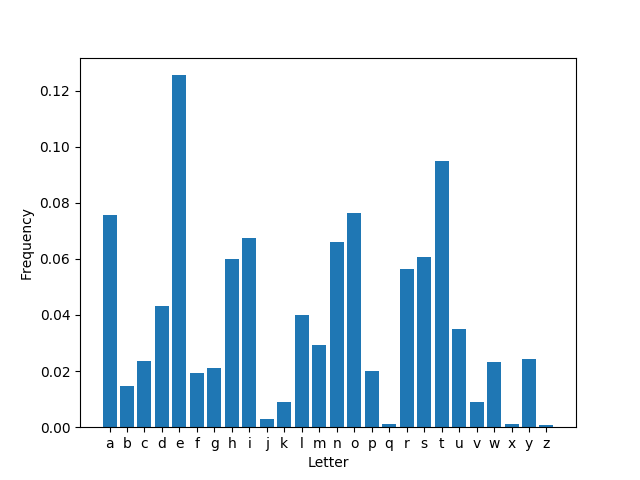
\includegraphics[width=0.5\columnwidth]{freq.png}
    \caption{Letter frequencies from \emph{The Secret Adversary} by Agatha
    Christie.}
    \label{fig:freq}
\end{figure}

\section{Polyalphabetic Substitution: The Vigen\`{e}re Cipher}

The next cipher, called the \emph{Vigen\`{e}re cipher} after its popularizer,
successfully defended against frequency analysis for hundreds of years. The
following description is informal, and I leave it to you to write a formal
definition like the above ciphers. A key for the cipher consists of some
finite number of ``shifts'' $K_1,K_2,\ldots,K_n$, each in $\{0,1,\ldots,25\}$.
To encrypt a string of letters, the cipher applies shift $K_1$ to the first
letter, then $K_2$ to the second, and so on up to applying $K_n$ to the
$n$\textsuperscript{th} letter. For the next letter, the first shift $K_1$
is reusued, and so on.

This cipher was particularly popular because it was both hard to break and easy
to use. Instead of numbers, one can represent the shifts using letters, and one
can even pick the shifts as a word. For instance, the key $K=\mathtt{MAROON}$
corresponds to shifts of $12,0,17,14,14,13$, but is easily remembered.

This type of cipher is called \emph{polyalphabetic} because it is using
``multiple alphabets'' in a systematic fashion. For even moderately
large $n$, exhaustive key search becomes impractically slow because
there are $26^n$ keys. Naive frequency analysis also fails, as the
frequencies get averaged over the different shifts.

\subsection{Breaking the Polyalphabetic Ciphers}

The cipher is still easily broken by modern standards, however. There are two
steps: Finding the key length $n$, and then finding the shifts. One method for
finding the key length is to simply try them all, starting from $n=1$, divide
the letters into buckets modulo $n$, and examine the frequencies within each
bucket. If you have the correct $n$ and enough text, then diagramming the
frequencies for each bucket should look like Figure~\ref{fig:freq}, but with
the columns cyclically permuted.

Another trick that works surprisingly well is called \emph{Kasiski Examination}.
here one looks for chunks of text that repeat will typically be spaced
by a multiple of $n$ apart. For example, in the ciphertext
\[
    \mathtt{C\underline{TYC}GST\underline{TYC}VOPRQBTBA\underline{TYC}LOURAPGBGIAPGQCEAPGG},
\]
the occurrences of $\mathtt{TYC}$ are spaced 6 and 12 apart; This suggests
that $n$ divides $6$, so probably $n\in\{1,2,3,6\}$.

A similar method tries moving the entire ciphertext forward by one spot, then
two, then three, etc, counting the number of characters that match between the
modified string and the original. Usually when the key length is reached,
there will be an unusually large number of matches.
For example, after moving everything forward
one spot, we find that two characters match:
\begin{align*}
    & \mathtt{CTYCGST\underline{\color{red}T}YCVOPRQBTBATYCLOURAPGBGIAPGQCEAPG\underline{\color{red}G}} \\
    & \mathtt{\phantom{\mathtt{X}}CTYCGS\underline{\color{red}T}TYCVOPRQBTBATYCLOURAPGBGIAPGQCEAP\underline{\color{red}G}G} 
\end{align*}
Shifts $2,3,4,5$ similarly produce a few matches, but
a shift of $6$ yields nine matching characters:
\begin{align*}
    & \mathtt{CTYCGST\underline{\color{red}TYC}VOPRQBTBATYCLOURAPGBGI\underline{\color{red}APG}QCE\underline{\color{red}APG}G} \\
    & \mathtt{\phantom{\mathtt{000000}}C\underline{\color{red}TYC}GSTTYCVOPRQBTBATYCLOUR\underline{\color{red}APG}BGI\underline{\color{red}APG}QCEAPGG} 
\end{align*}
One would tend to guess that $6$ is the key length.

Once the key-length has been recovered, the rest of the attack is simple
and mostly left to you. The crucial fact is that for each bucket there
are only a small number of possible shifts, and one of them should cycle
the frequencies around to closely match the frequencies typical English.

\section{Homophonic Substitution}

Another method for defeating frequency analysis is to allow multiple possible
representations of the same message letter. I'll again describe an example of
this cipher informally.  The example cipher takes $\msgs = \Sigma^+$ as before,
but it lets $\ctxts = (\Sigma\cup\Pi)^+$, where $\Pi =
\{\mathtt{0},\mathtt{1},\ldots,\mathtt{9}\}$ are digits.  A typical key
will look the following table:

\begin{small}
\begin{tabular}{*{26}{c}}
    \texttt{A} &
    \texttt{B} &
    \texttt{C} &
    \texttt{D} &
    \texttt{E} &
    \texttt{F} &
    \texttt{G} &
    \texttt{H} &
    \texttt{I} &
    \texttt{J} &
    \texttt{K} &
    \texttt{L} &
    \texttt{M} &
    \texttt{N} &
    \texttt{O} &
    \texttt{P} &
    \texttt{Q} &
    \texttt{R} &
    \texttt{S} &
    \texttt{T} &
    \texttt{U} &
    \texttt{V} &
    \texttt{W} &
    \texttt{X} &
    \texttt{Y} &
    \texttt{Z} \\
\hline
    \texttt{D} &
    \texttt{A} &
    \texttt{6} &
    \texttt{V} &
    \texttt{3}&
    \texttt{7}&
    \texttt{K}&
    \texttt{E}&
    \texttt{W}&
    \texttt{1}&
    \texttt{2}&
    \texttt{8}&
    \texttt{F}&
    \texttt{Z}&
    \texttt{J}&
    \texttt{T}&
    \texttt{P}&
    \texttt{5}&
    \texttt{U}&
    \texttt{Q}&
    \texttt{M}&
    \texttt{H}&
    \texttt{N}&
    \texttt{9}&
    \texttt{4}&
    \texttt{G} \\

    \texttt{C} &
    &
    &
    &
    \texttt{B} &
    &
    &
    \texttt{Y} &
    \texttt{S} &
    &
    &
    &
    &
    \texttt{I} &
    \texttt{X} &
    &
    &
    \texttt{R} &
    \texttt{L} &
    \texttt{0} \\
    &
    &
    &
    &
    \texttt{O}
\end{tabular}
\end{small}

Now encryption is defined to map each letter to \emph{one of} the letters
listed below it. For \texttt{A} there are two choices: \texttt{D} and
\texttt{C}, while \texttt{C} will always map to \texttt{6}. When multiple
options are available, encryption can pick arbitrarily. For instance, it
can rotate amongst the choices, or even pick a choice at random each
time.\footnote{Strictly speaking, if we allow $\enc$ to pick options at
random, then it is no longer a function; It's a sort of ``randomized
function'', where the output $\enc(K,M)$ is a random variable.}

The output options may be much larger than 36. For instance, in the
Great Cipher, each letter was mapped to a three digit number.

\subsection{Breaking the Homophonic Ciphers}

A properly designed homomophonic cipher can make frequency analysis perform
very poorly, since it evens out the distribution of most of the letters.
However, with a large enough ciphertext some patterns emerge. Once the output
alphabet has been determined, one useful technique is to analyze the frequency
of \emph{pairs} or \emph{triples} (usually called bigrams and trigrams) of
consecutive outputs.  In a large text, commmon bigrams and trigrams will
eventually emerge as (less common) bigrams and trigrams in the ciphertext. By
starting with the most frequent bigrams and trigrams, one can start guessing
substitutions and checking if a consistent text emerges.

\section{The One-Time Pad Cipher}

This last cipher gets a new name, but it is just the Vigen\'{e}re cipher
with a very large key; In fact, as large as the message that is being
sent. A bit more formally, this cipher will a message space
$\msgs = \Sigma^\ell$ for some fixed length $\ell$. It will also
take $\keys=\ctxts=\Sigma^\ell$ as well. The actual encryption
is defined exactly like Vigen\`{e}re (where we take the letters
of the key to represent shifts).

\subsection{Breaking the One-Time Pad Cipher}

Breaking the one-time pad is quite an interesting question. We'll return
to this later, but it turns out to be impossible in some circumstances!
One circumstance where it \emph{is} possible is when two messages are
encrypted with the same key. The key observation is that one can get
some information about the underlying messages in this case, and sometimes
enough to recover the entire messages.

Suppose that $C=\enc(K,M)$ and $C'=\enc(K,M')$
with $M\neq M'$ are both encrypted with the one-time pad cipher with same
key $K$. 
Use subscripts like $M_i$ to indicate the $i$\textsuperscript{th}
letter of a string, and let us treat letters interchangeably with
numbers modulo $26$.
Then
\[
    C_i - C'_i = (M_i+K_i) - (M'_i+K_i) = M_i - M'_i \mod 26,
\]
so one can learn $M_i-M'_i\mod 26$ from just the ciphertexts.
With some experimentation, it sometimes possible to run frequency analysis
on these differences, which will follow a general trend of the language.
Another approach, called \emph{crib-dragging}, is also commonly used
and can be found in other course material to be posted.

\end{document}

